\subsubsection{User Interfaces}

The user will be able to interact with the system via a web interface and a mobile application, available for all major browsers and mobile operating systems. These two views will be optimized for different screen sizes and different scenarios of use (e.g. a 24 inch pc display in an office or a 5 inch display on a phone outside), but they will share a clean and modern look together with the same color scheme.
\\ [0.2 cm]
Below you can find some example mockups that show a part of the user interface; they are not intended to be a complete and exhaustive set, but rather to act as a guide for future implementation.
\\ [0.5 cm]

\vspace*{-1cm}
\begin{figure}[!h]
	\centering
	\begin{minipage}{.275\textwidth}
		\centering
		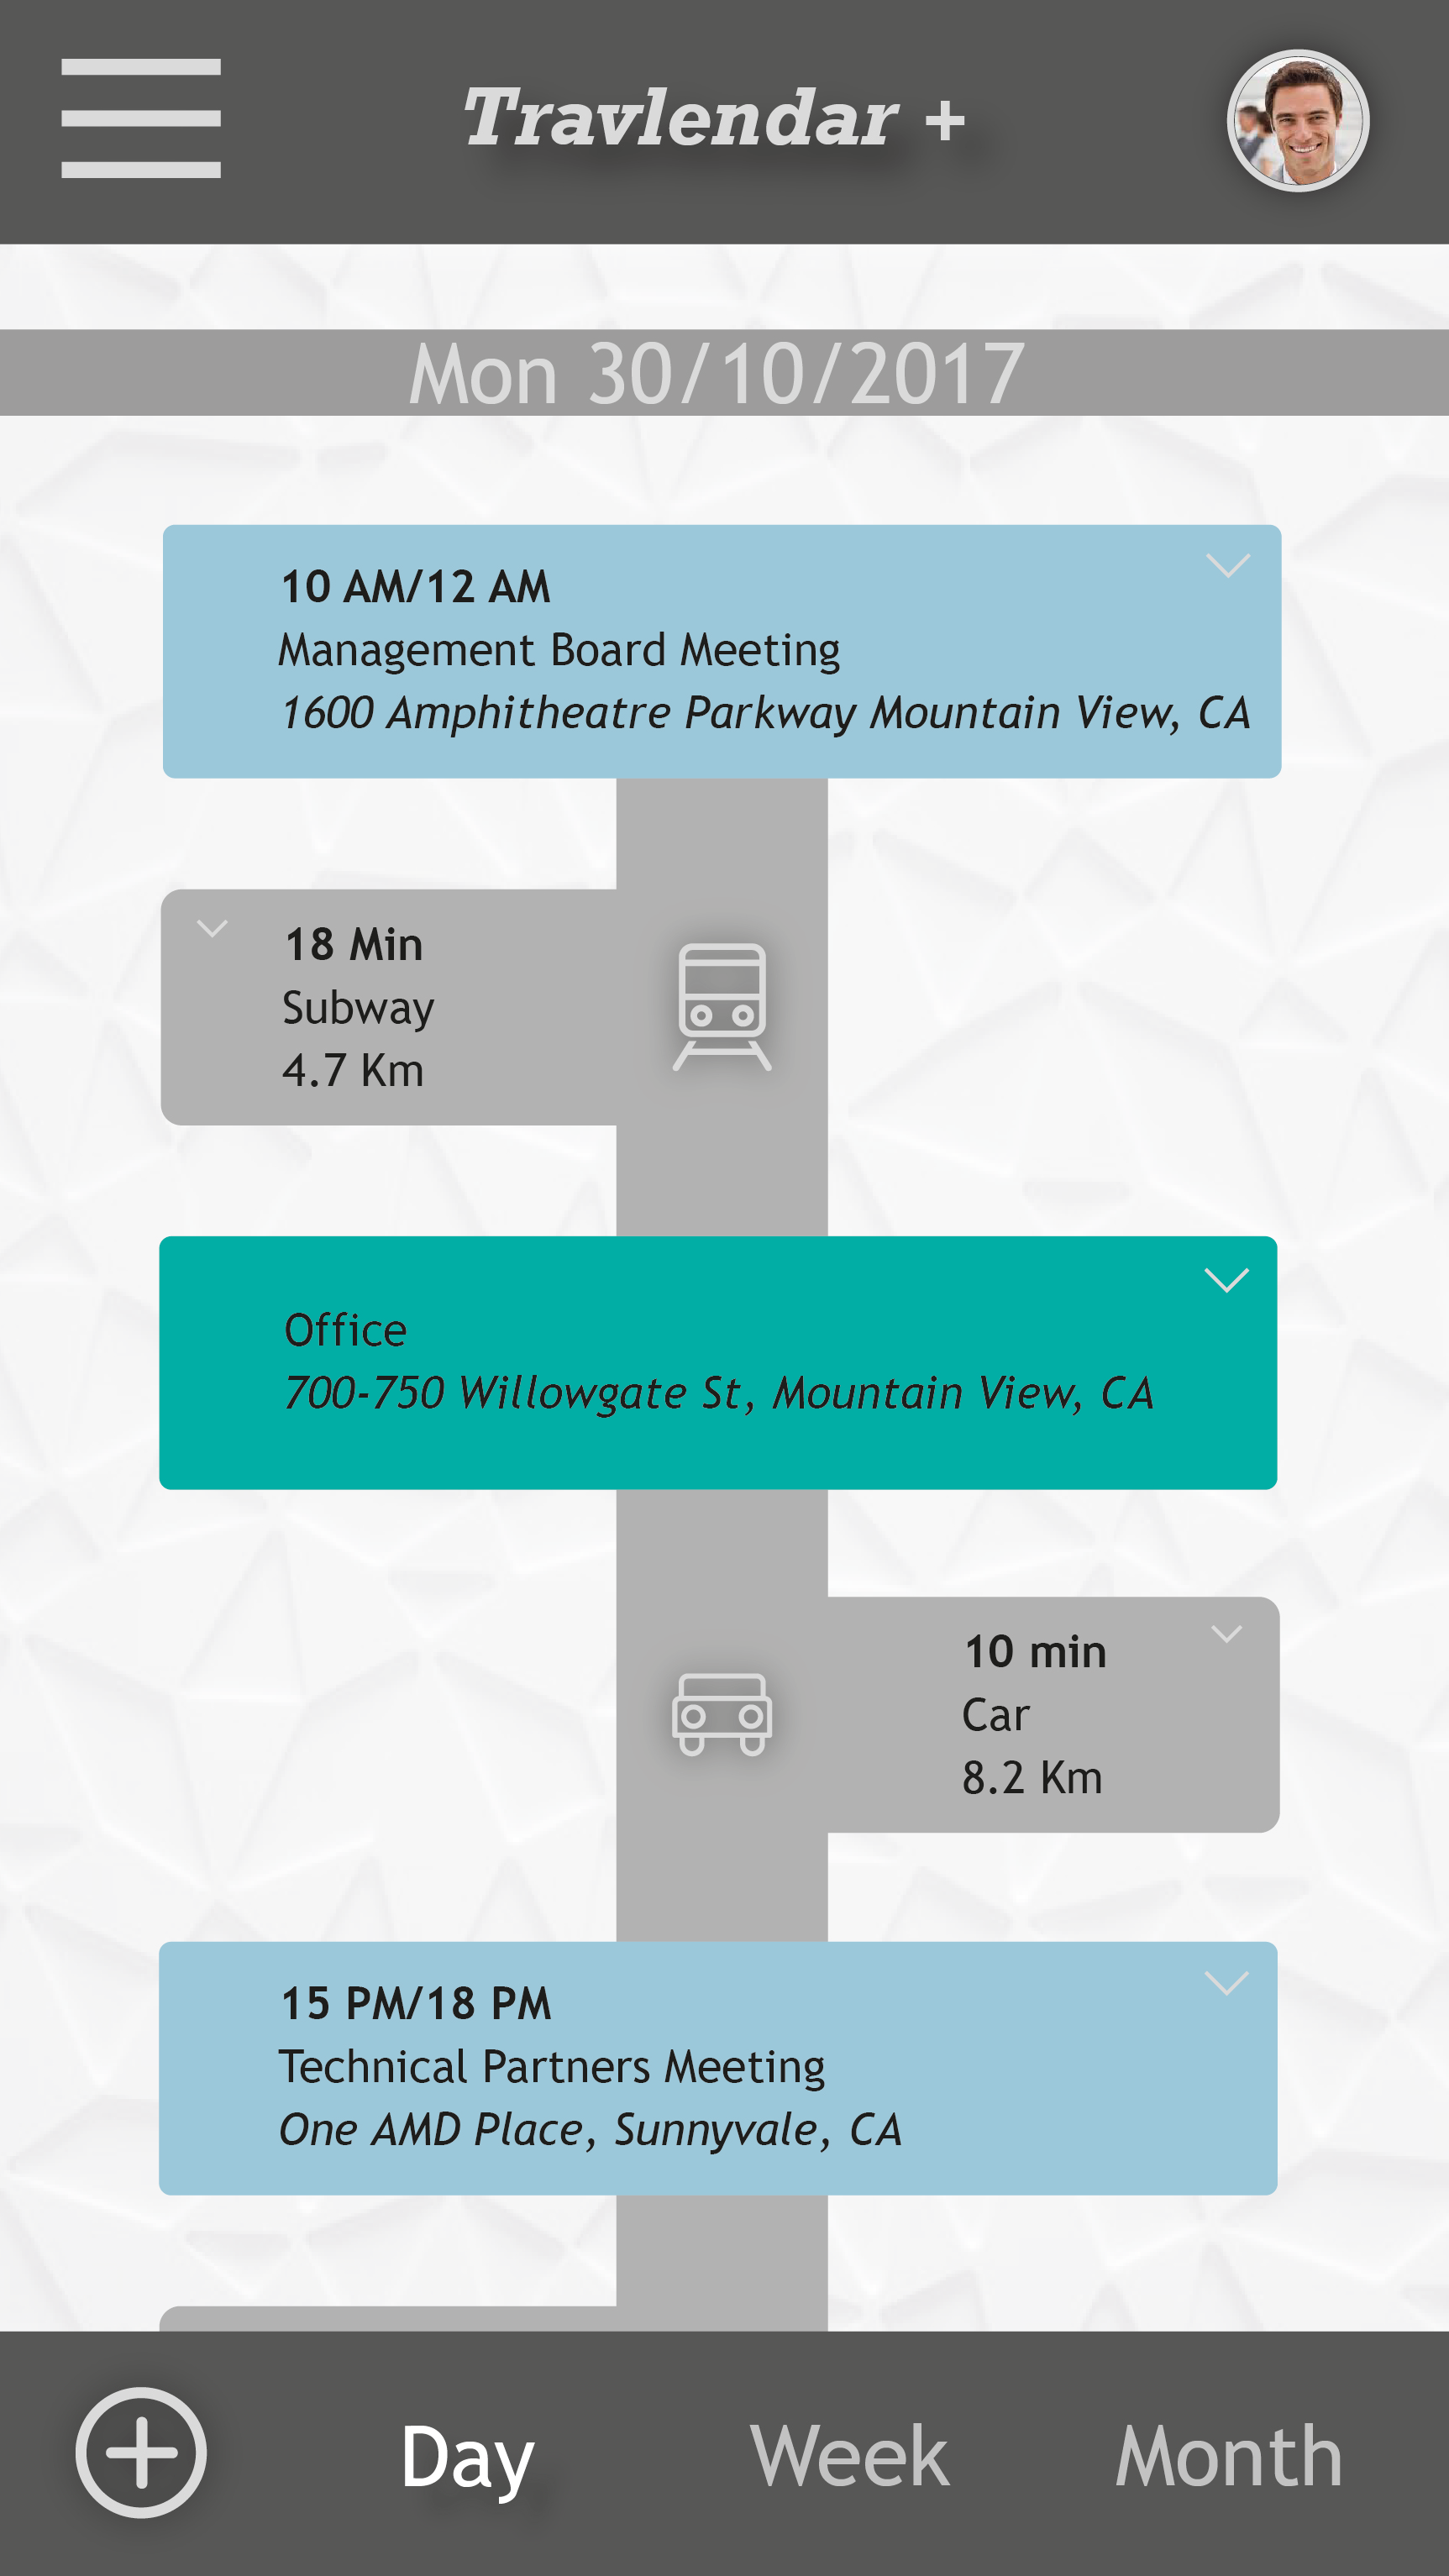
\includegraphics[width=\linewidth]{Images/Mockups/MockupCalendarApp.png}
		\caption{App Calendar}
	\end{minipage}%
	\hspace*{1cm}
	\begin{minipage}{.65\textwidth}
		\centering
		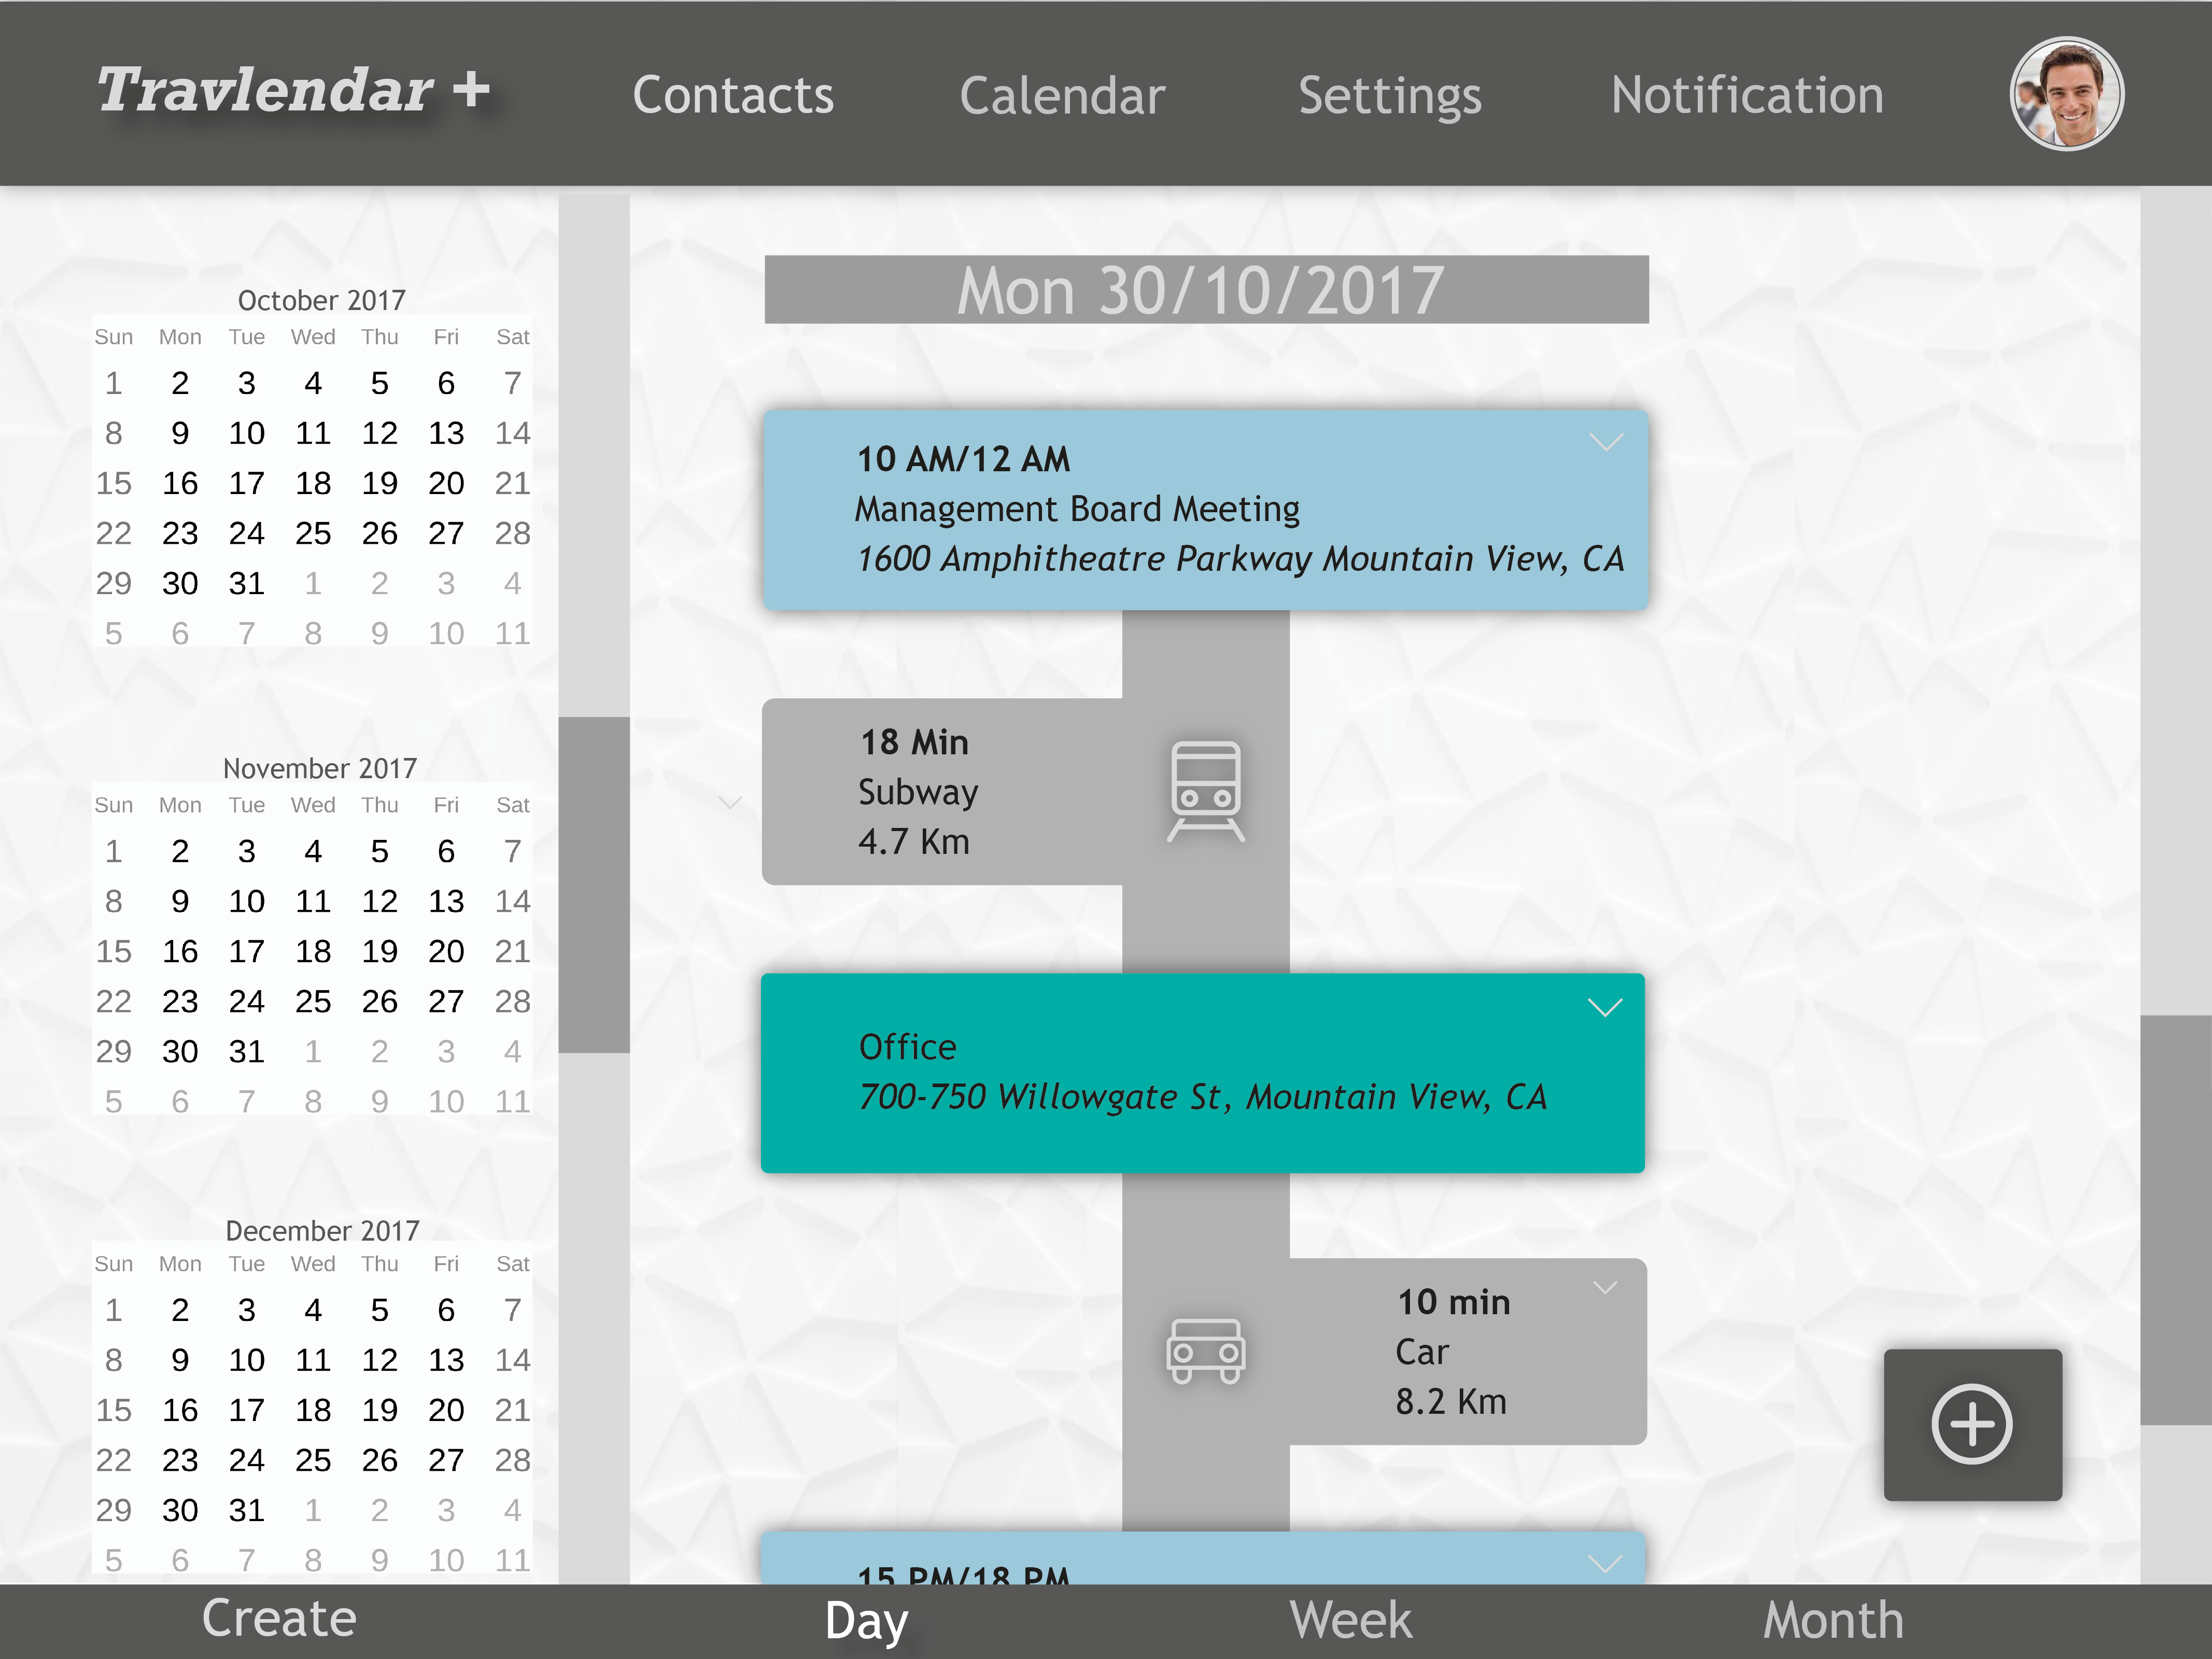
\includegraphics[width=\linewidth]{Images/Mockups/MockupCalendarWeb.png}
		\caption{Web Calendar}
	\end{minipage}
\end{figure}

\vspace*{-0.2cm}
\begin{figure}[!h]
	\centering
	\begin{minipage}{.275\textwidth}
		\centering
		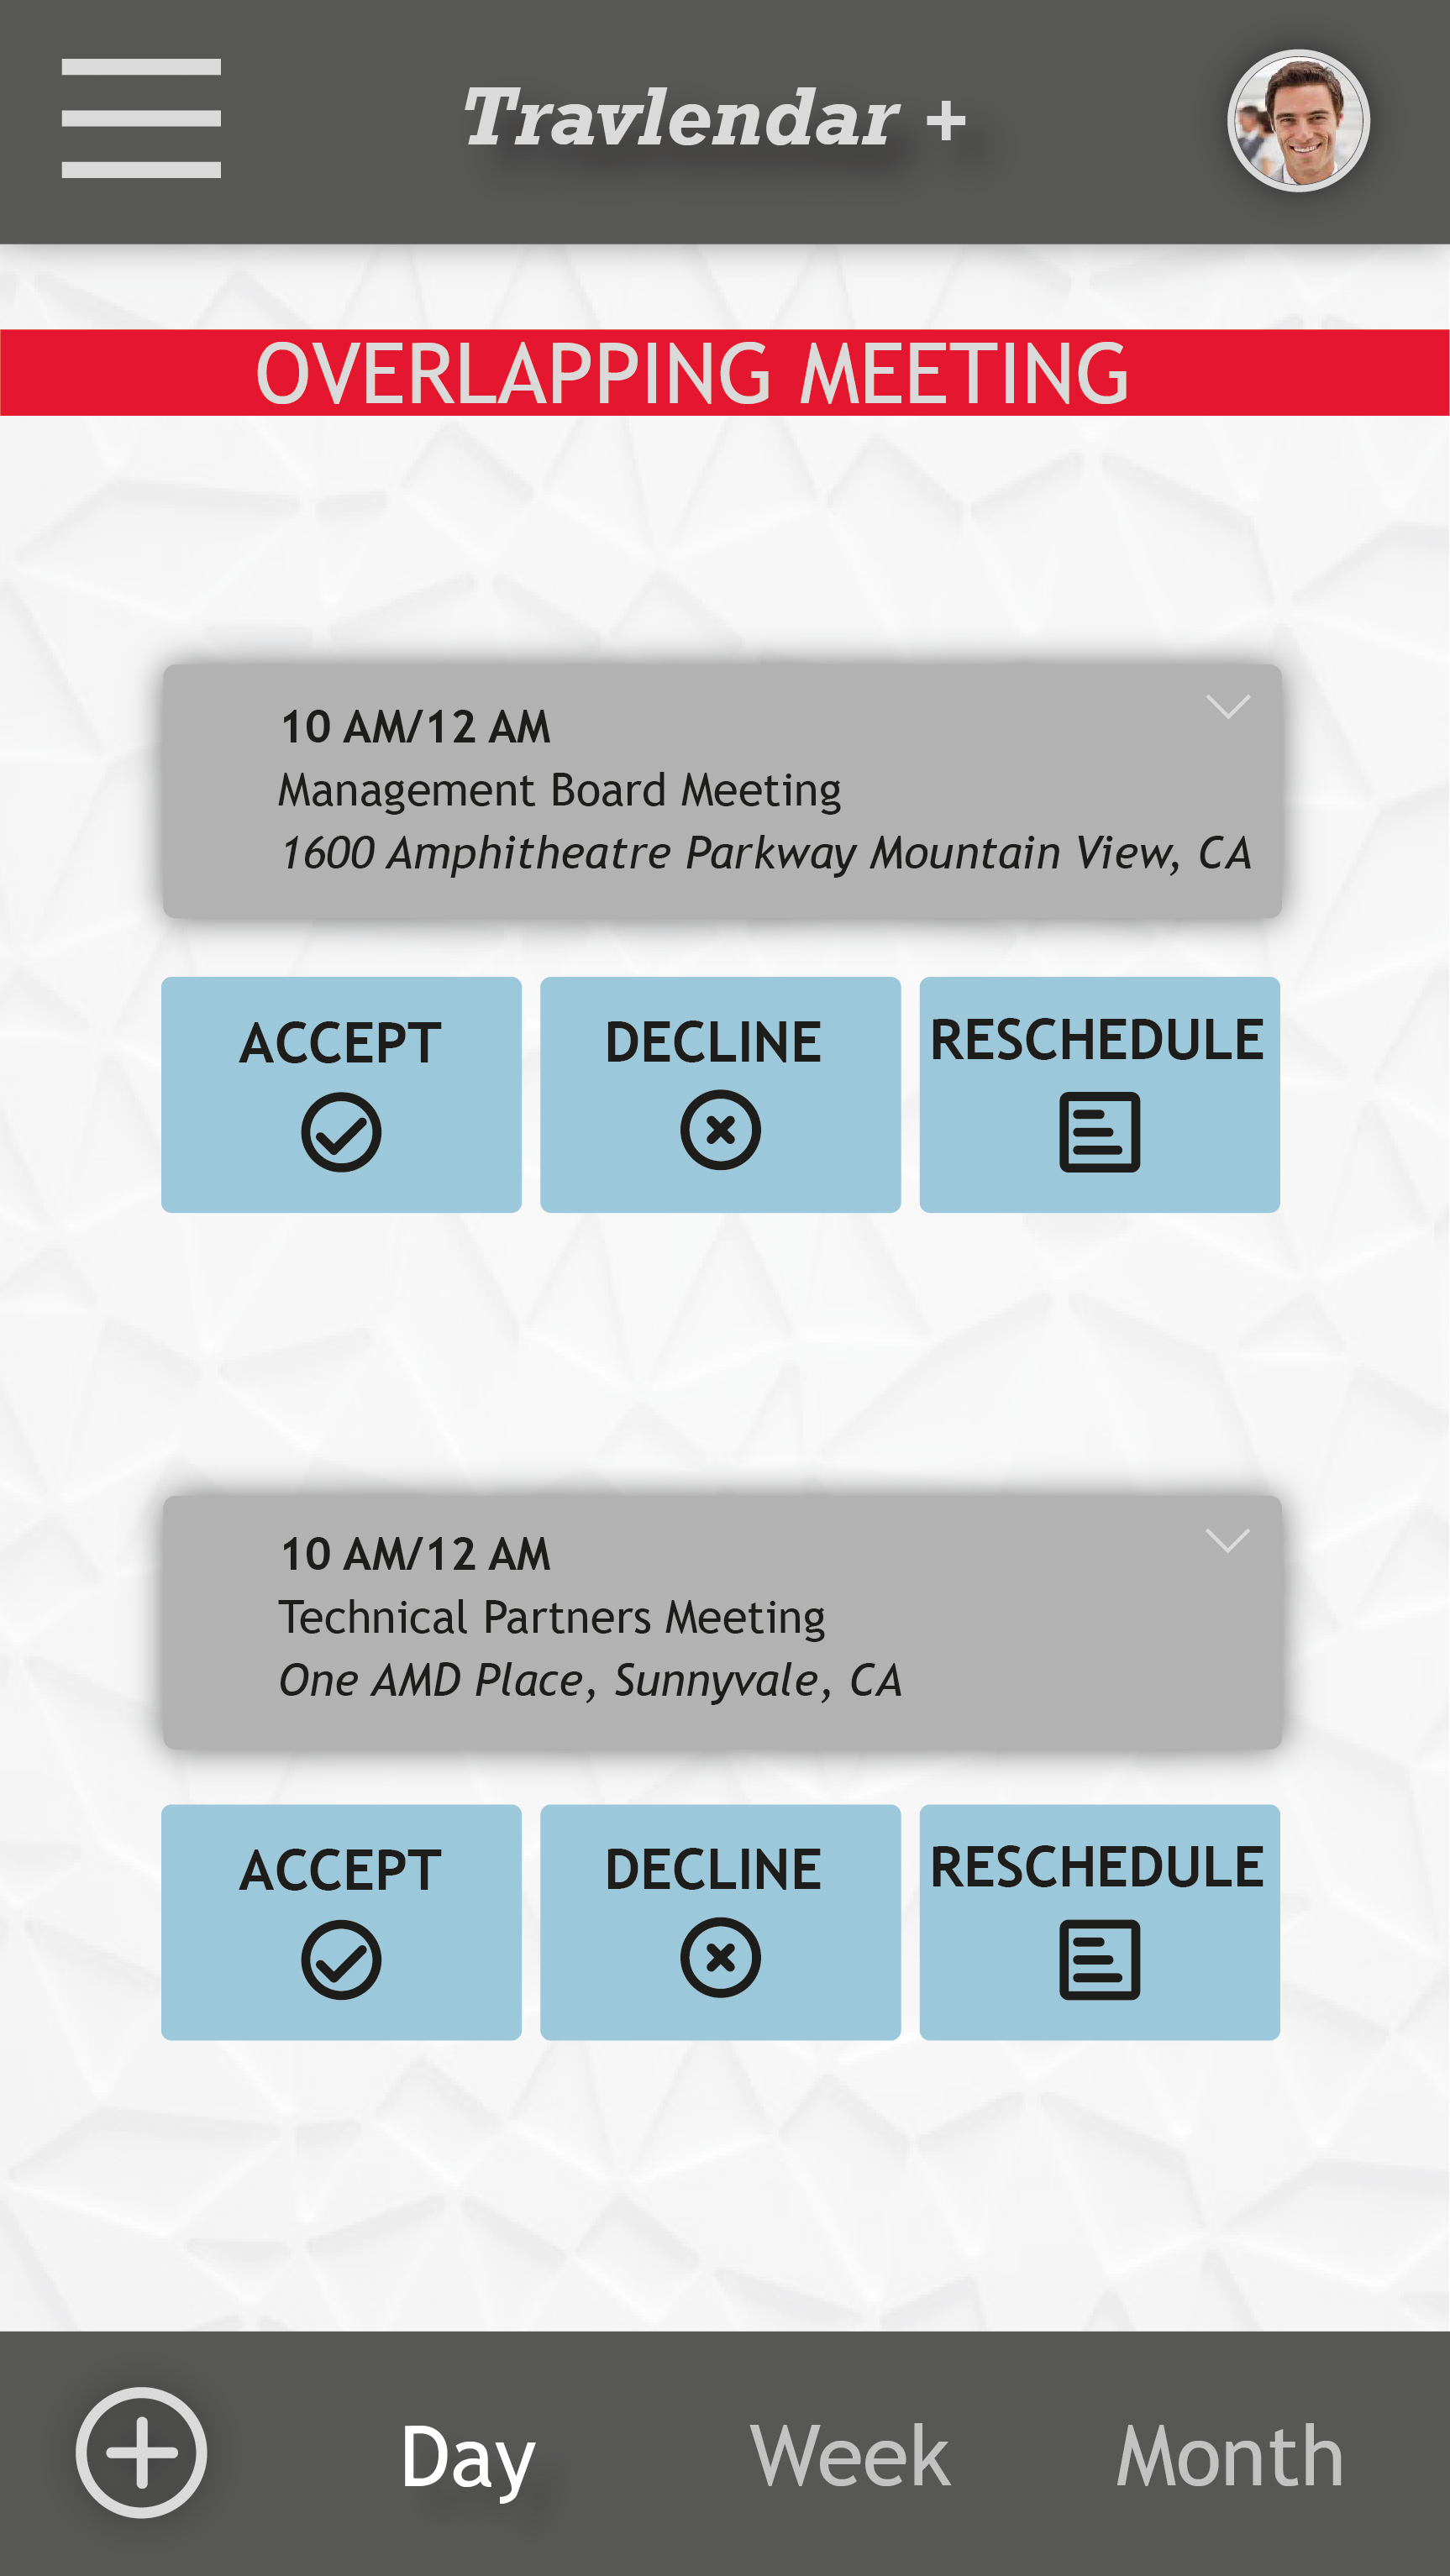
\includegraphics[width=\linewidth]{Images/Mockups/MockupWarningApp.png}
		\caption{App Warning}
	\end{minipage}%
	\hspace*{1cm}
	\begin{minipage}{.65\textwidth}
		\centering
		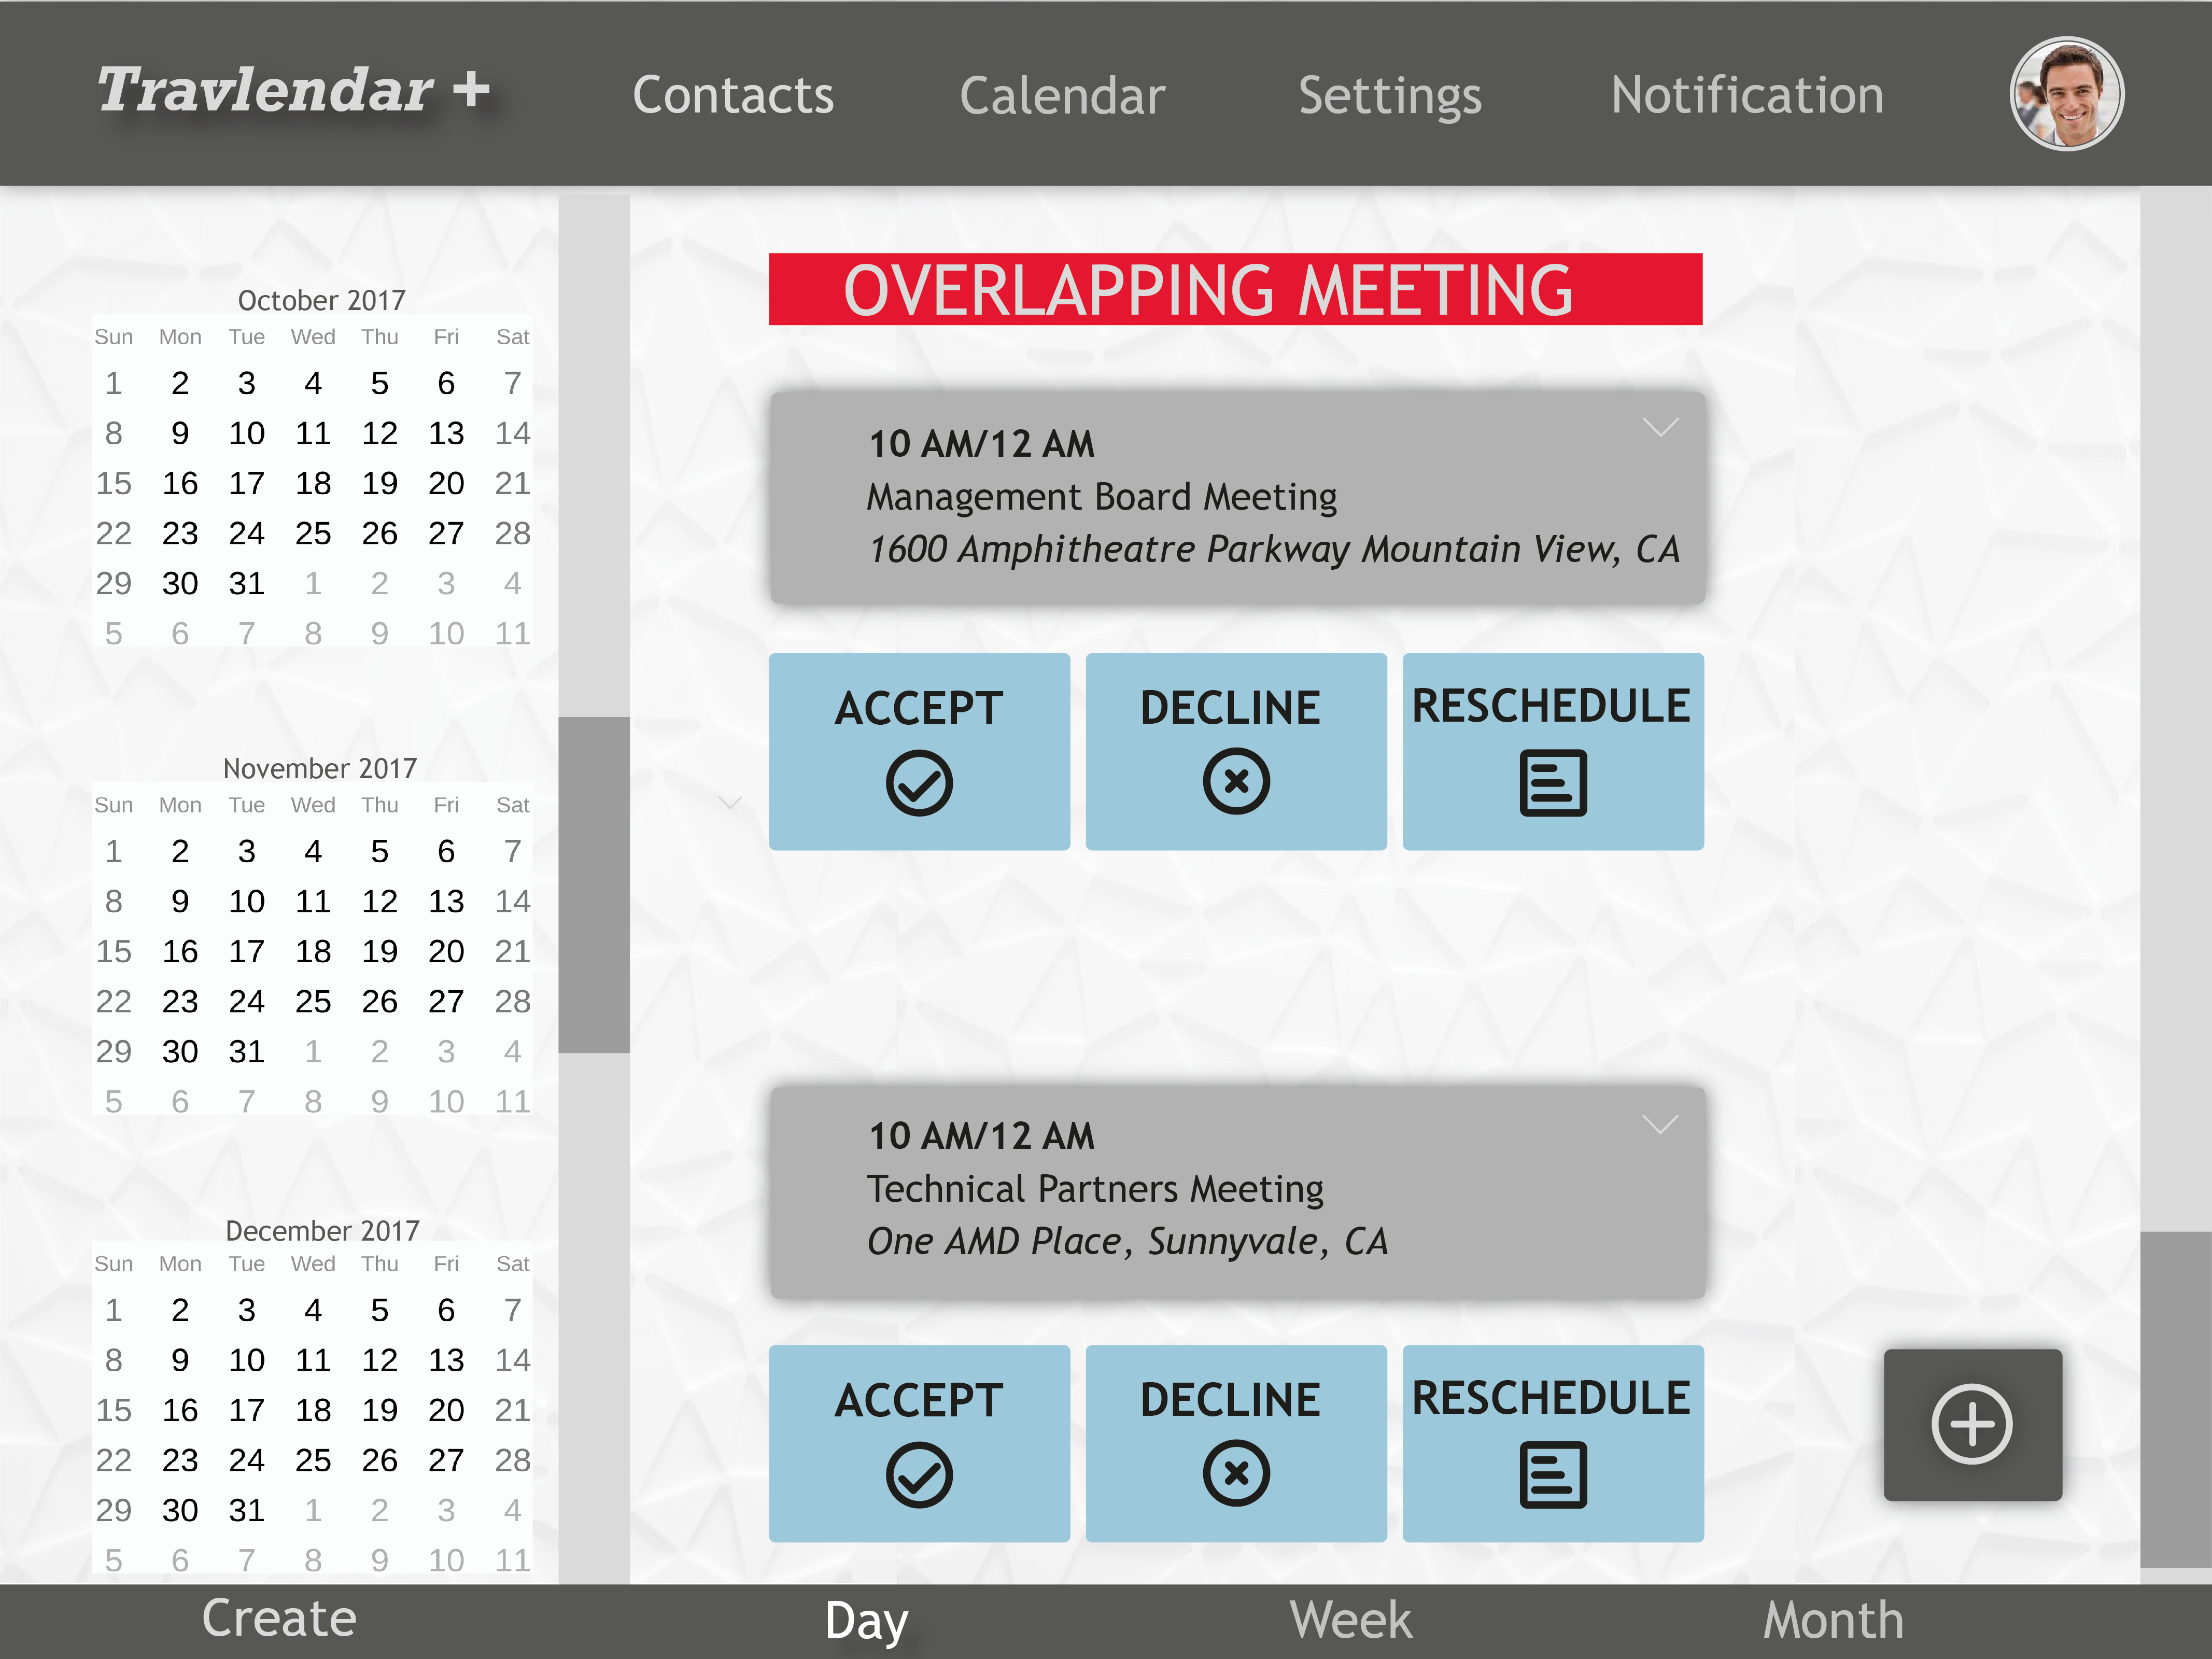
\includegraphics[width=\linewidth]{Images/Mockups/MockupWarningWeb.png}
		\caption{Web Warning}
	\end{minipage}
\end{figure}

\begin{figure}[!h]
	\centering
	\begin{minipage}{.275\textwidth}
		\centering
		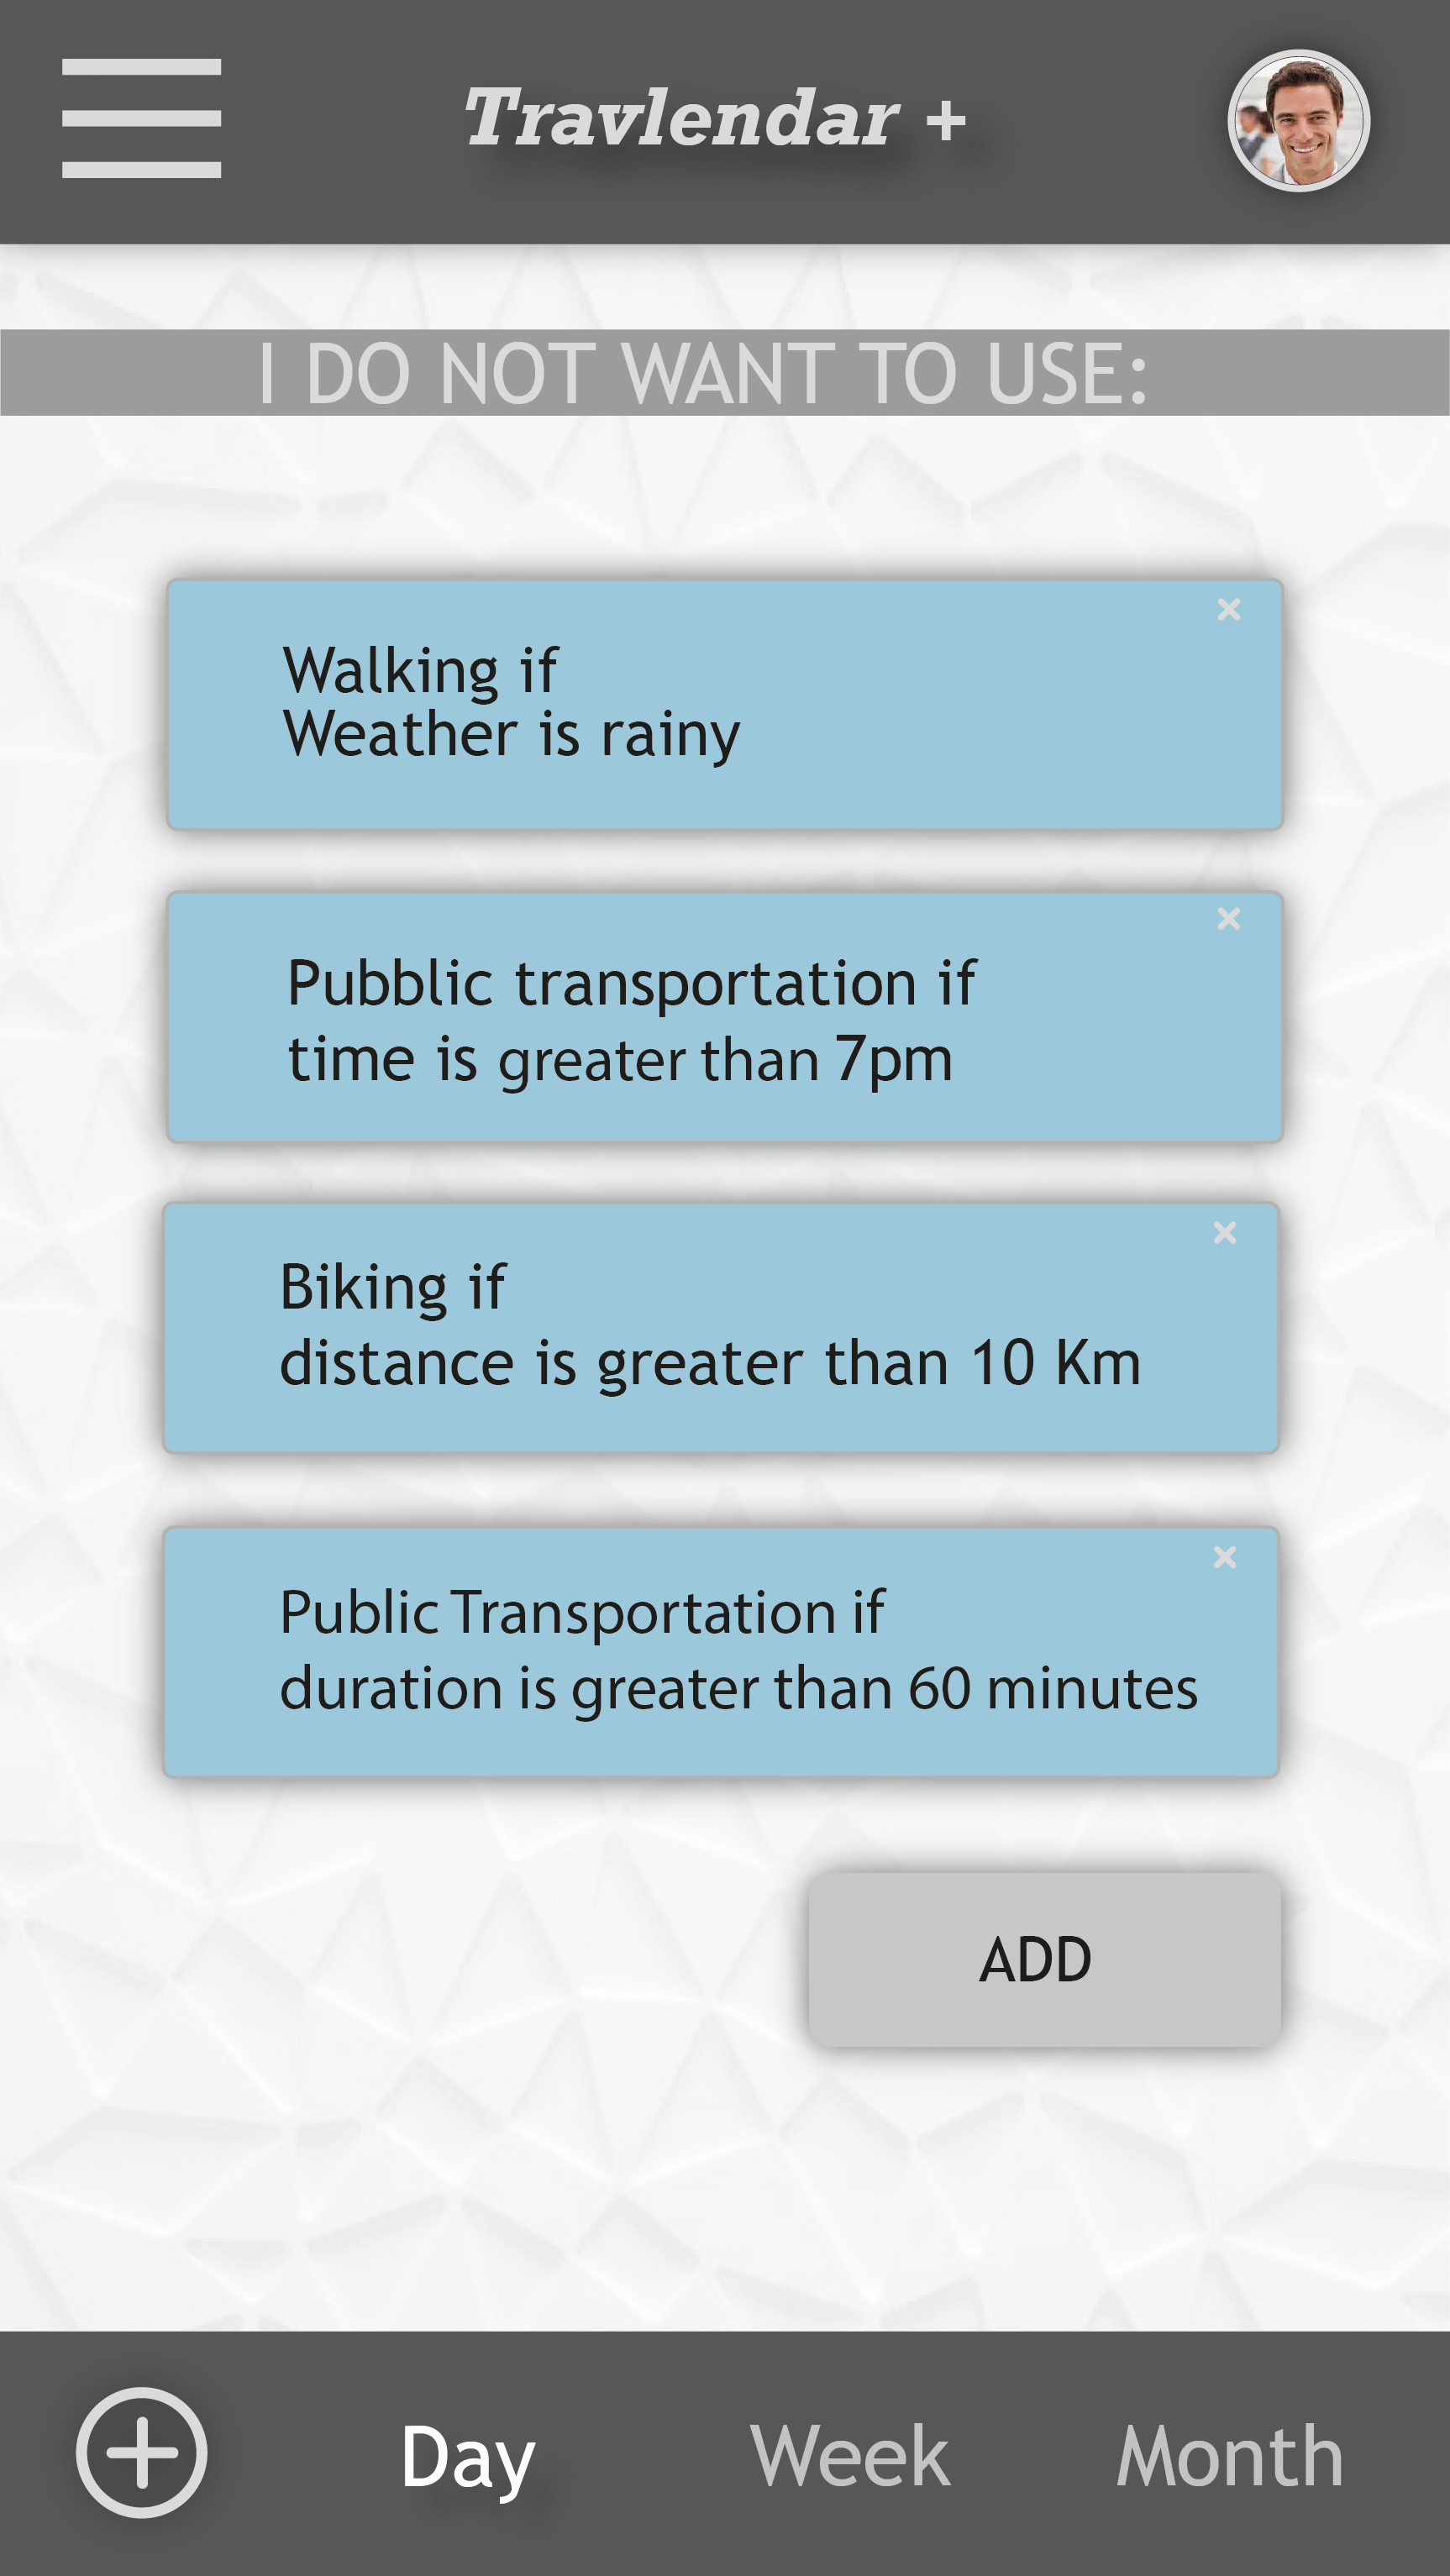
\includegraphics[width=\linewidth]{Images/Mockups/MockupConstraintsApp1.png}
	\end{minipage}%
	\hspace*{1cm}
	\begin{minipage}{.275\textwidth}
		\centering
		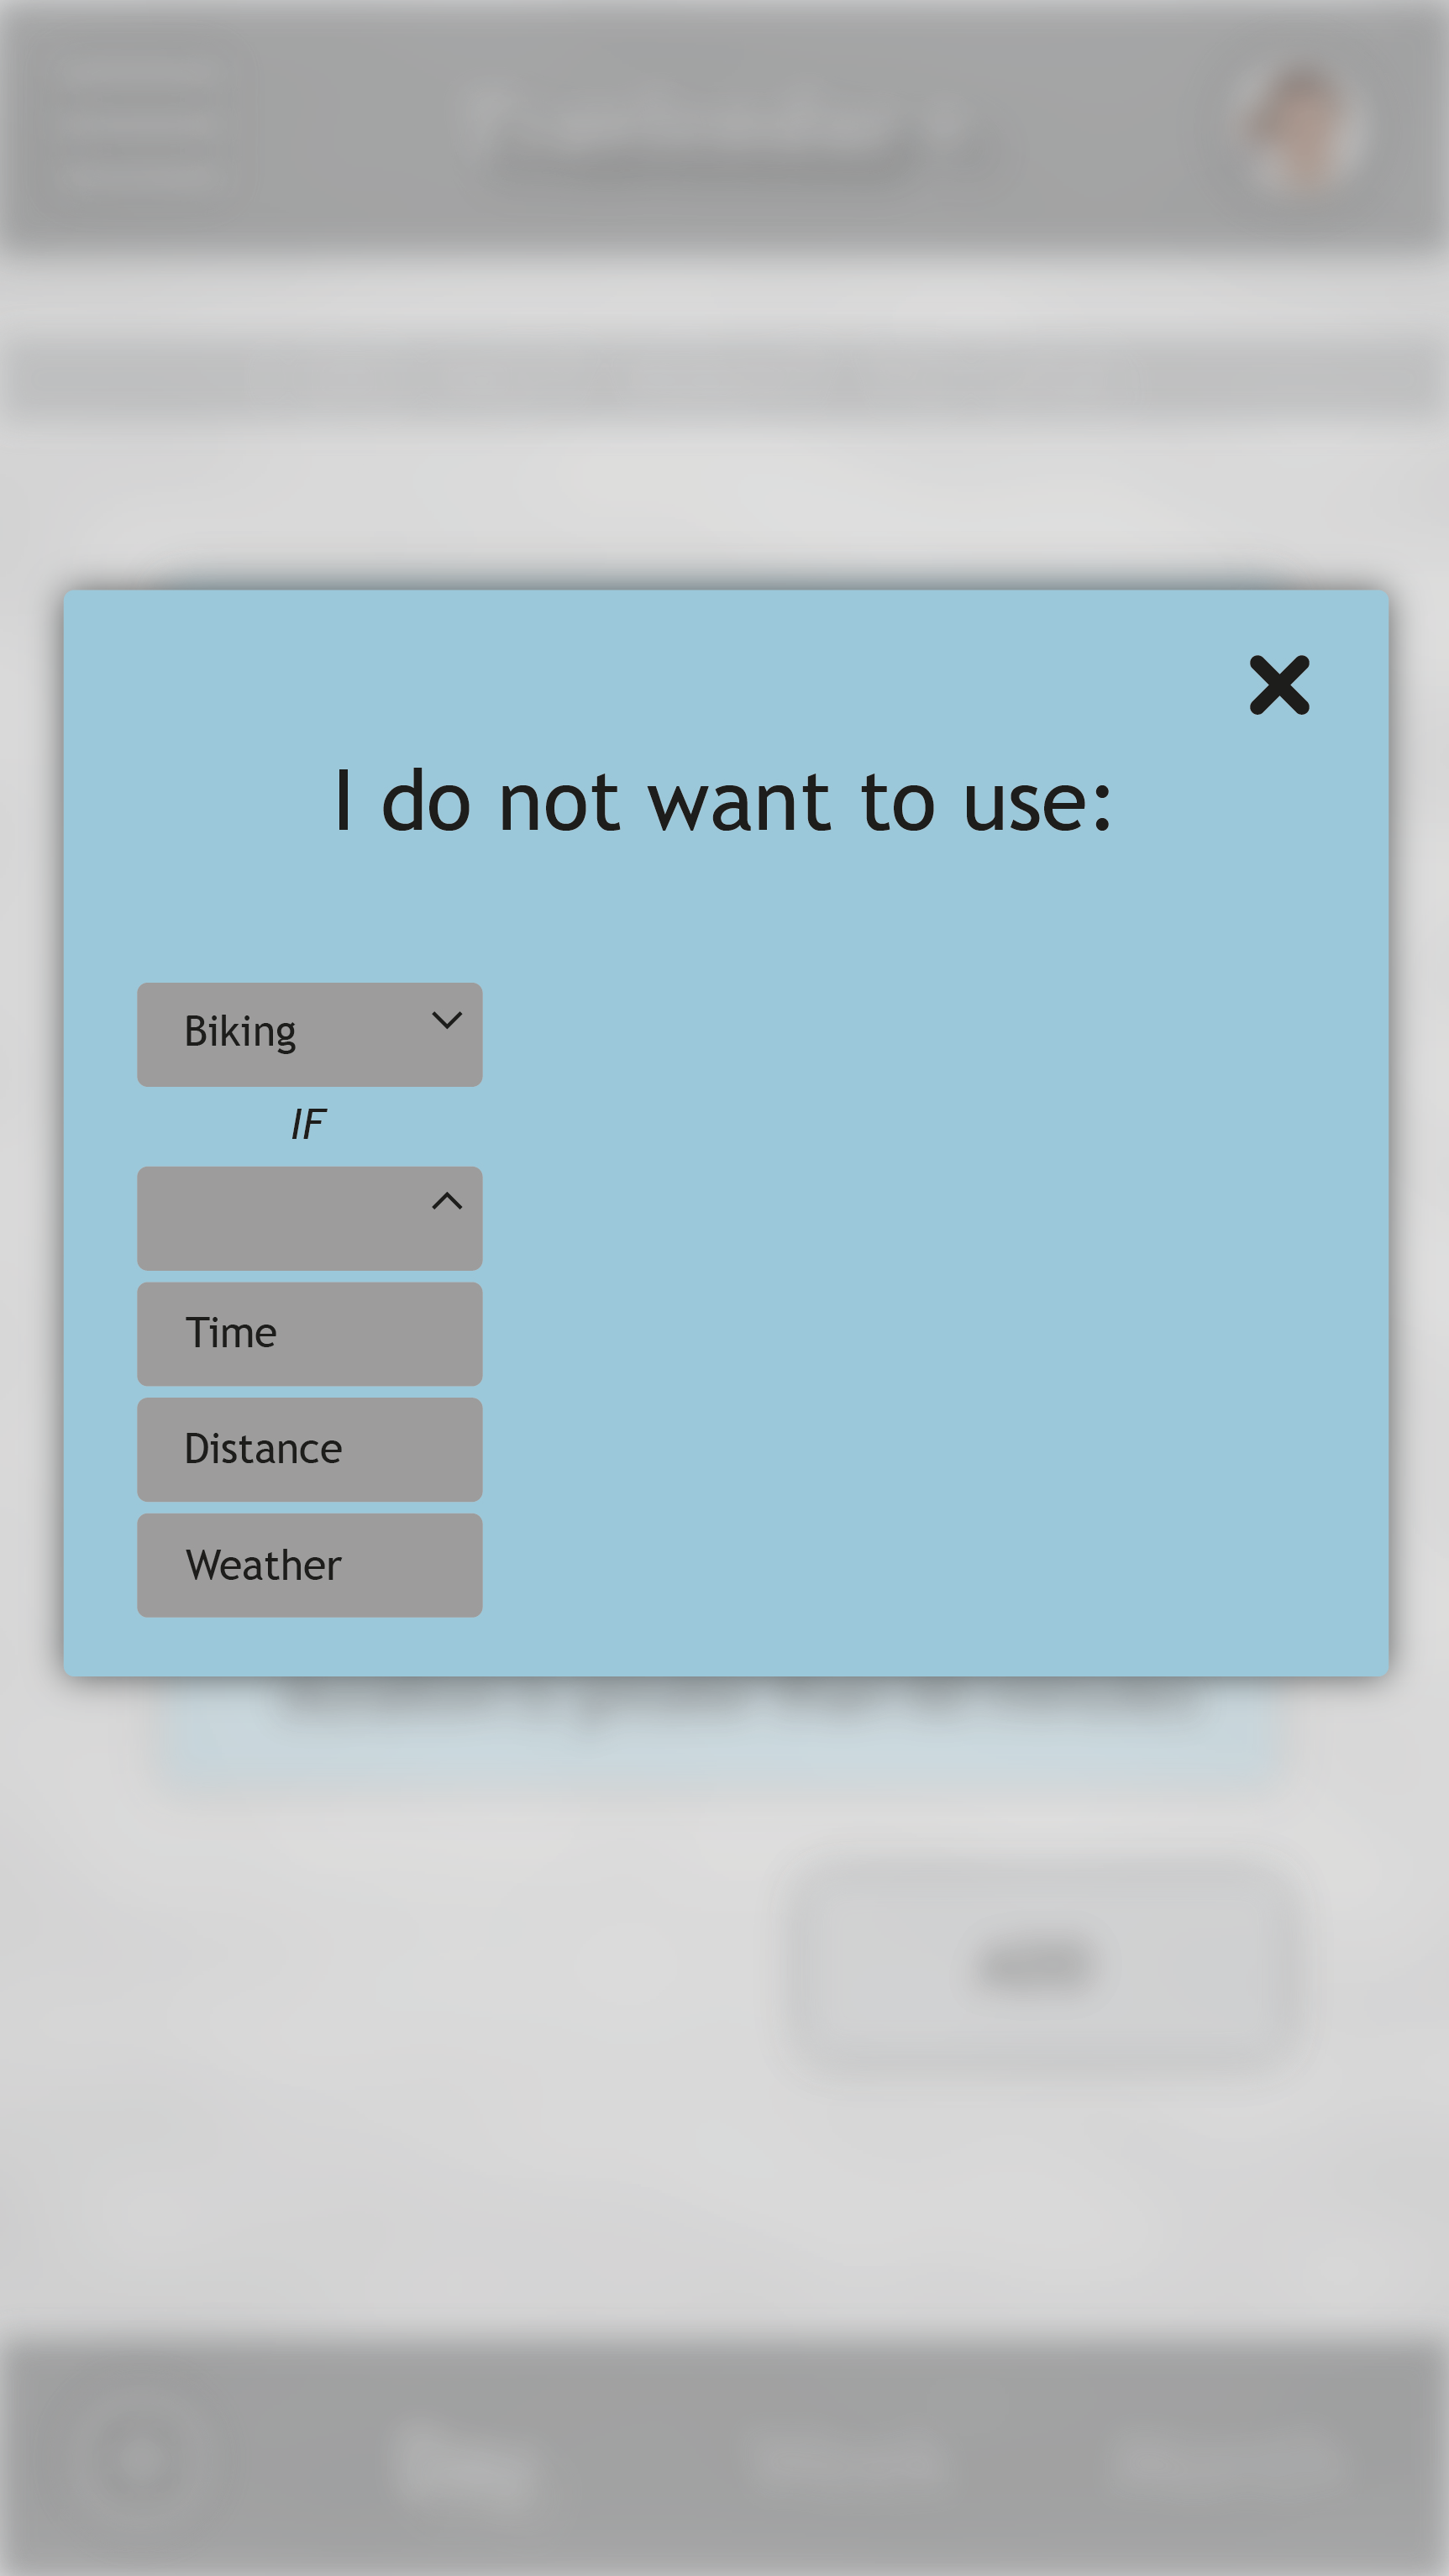
\includegraphics[width=\linewidth]{Images/Mockups/MockupConstraintsApp2.png}
	\end{minipage}
	\hspace*{1cm}
	\begin{minipage}{.275\textwidth}
		\centering
		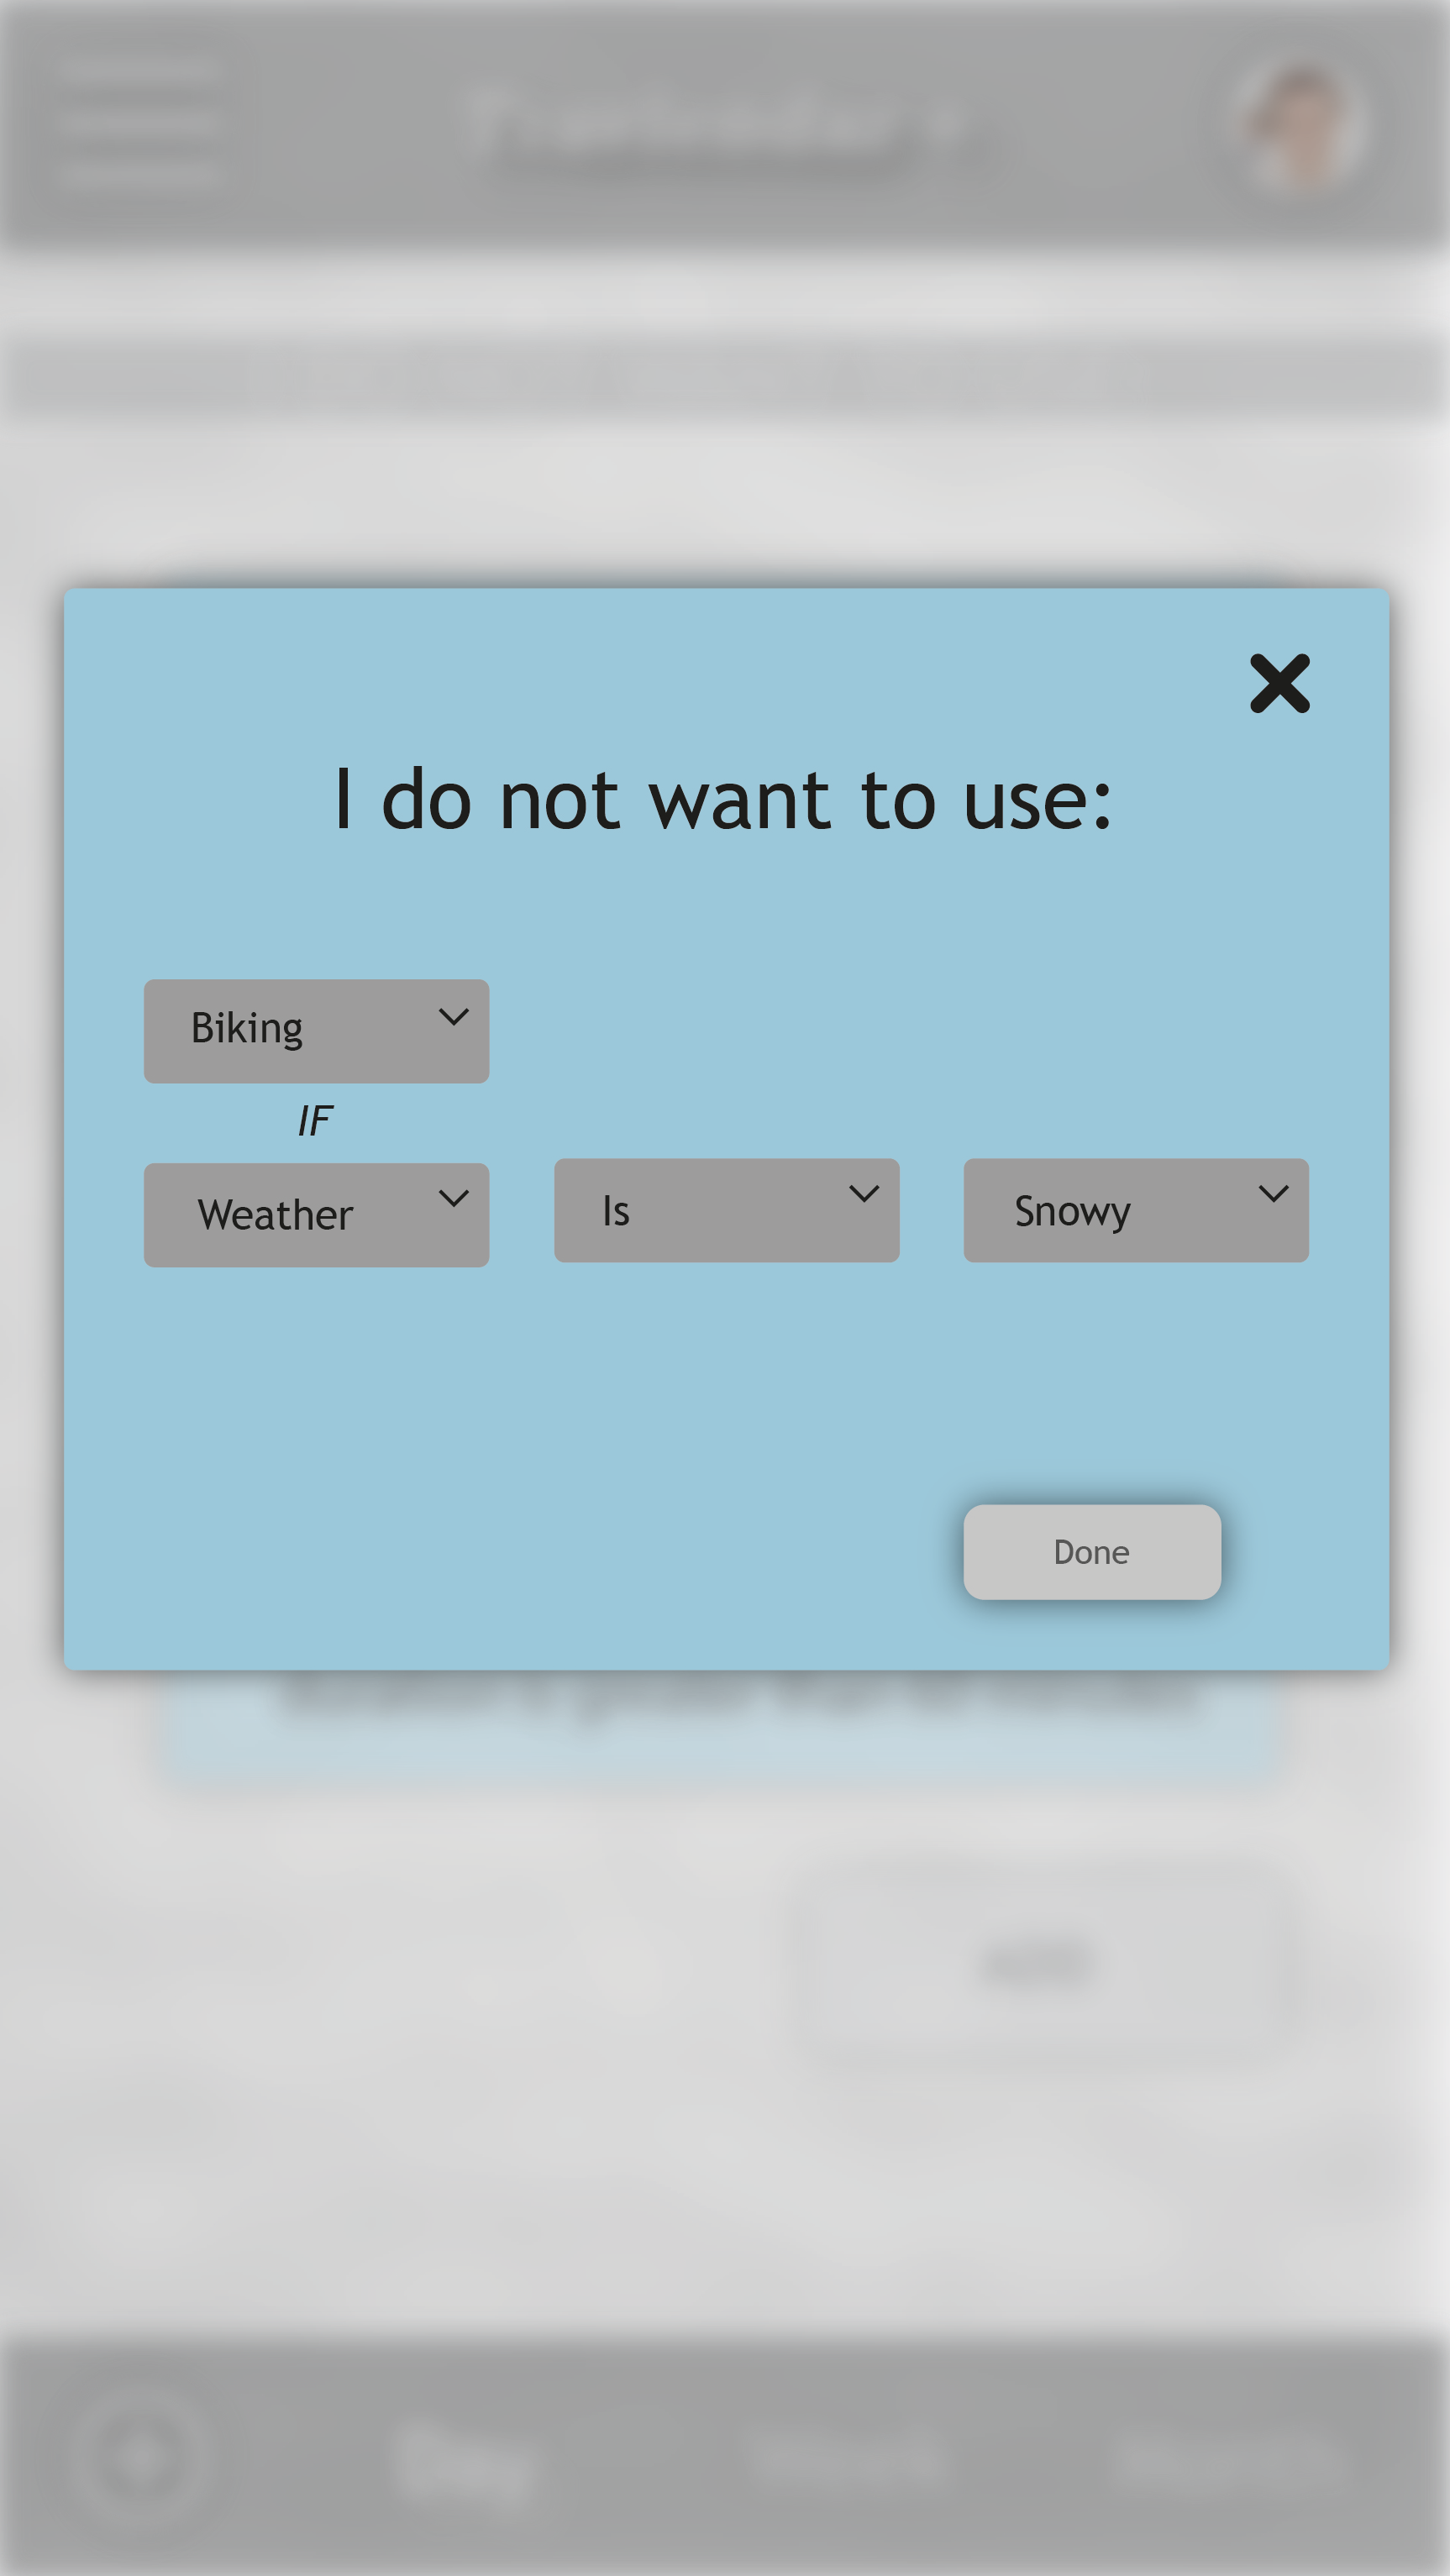
\includegraphics[width=\linewidth]{Images/Mockups/MockupConstraintsApp3.png}
	\end{minipage}
	\caption{App Constraints}
\end{figure}

\subsubsection{Hardware Interfaces}

The system won't include any particular or dedicated hardware, and so no interface has to be devised.


\subsubsection{Software Interfaces}
The system will need to interact with a data management system, with external login providers and with an external shortest path provider.\\
For the first one, one of the many relational database on the market will be chosen as they all generally meet the needs of this project; a library or a framework will be used to interface with it, in accordance to the design and implementation choices that will be made.\\
As regards external login providers, the main ones will be supported in order to reach as many users as possible without too much development effort; the interface with them is usually dependent on the particular provider, so they have to be implemented on a case by case basis, perhaps with the help of a library.\\
For the external shortest path provider, a single one will be chosen to handle all different travel means in order to have to manage a single interface.

\subsubsection{Communication Interfaces}

The system won't include any particular communication protocol, and so no interface has to be devised. For client-server communication we will use plain HTTP.